\chapter{Joshua 18}

\begin{figure}
  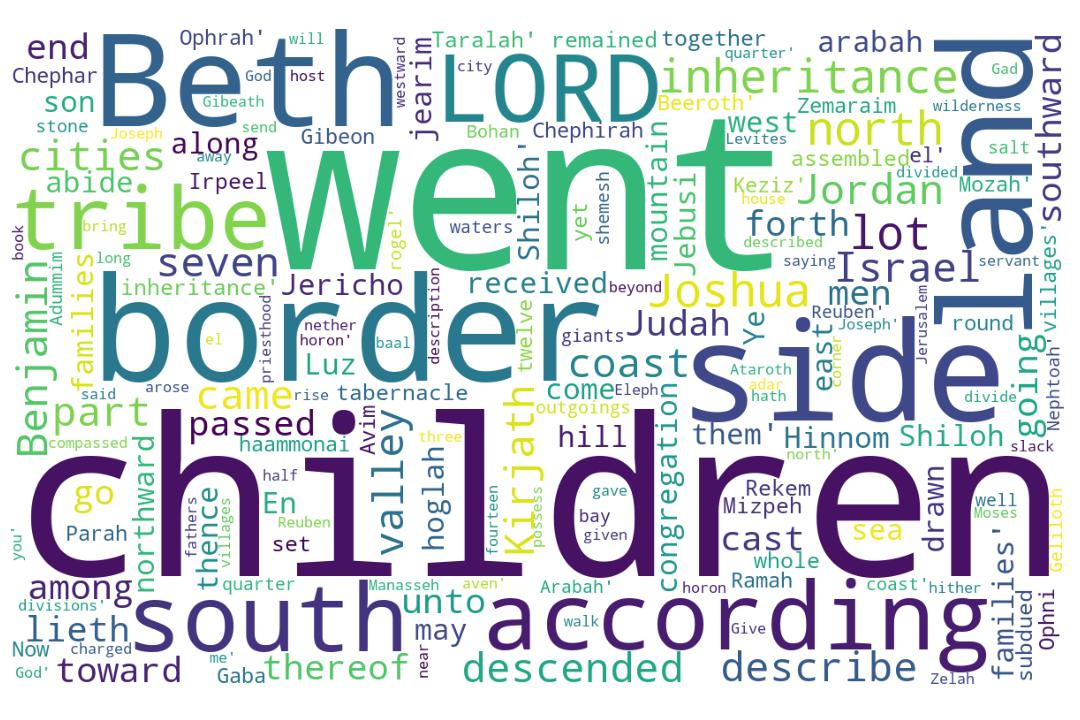
\includegraphics[width=\linewidth]{06OT-Joshua/Joshua18-WordCloud.jpg}
  \caption{Joshua 18 Word Cloud}
  \label{fig:Joshua 18 Word Cloud}
\end{figure}


\marginpar{\scriptsize \centering \fcolorbox{bone}{lime}{\textbf{LAND FOR BENJAMIN}}\\ (Joshua 18:1-28) \begin{compactenum}[I.][8]
	\item A Land \textbf{Subdued}  \index[scripture]{Joshua!Jsh 18:01} (Jsh 18:1) 
	\item A \textbf{Slackness}  \index[scripture]{Joshua!Jsh 18:03} (Jsh 18:3) 
	\item The \textbf{Scouts}  \index[scripture]{Joshua!Jsh 18:04} (Jsh 18:4) 
	\item  \textbf{Seven} Portions \index[scripture]{Joshua!Jsh 18:05} (Jsh 18:5) 
	\item The \textbf{Specfics}  \index[scripture]{Joshua!Jsh 18:11--28} (Jsh 18:11--28) 
	\item A Solid \textbf{Strategy} for Decisions -- analysis, counsel, prayer % \index[scripture]{Joshua!Jsh 18:11--28} (Jsh 18:11--28) 
\end{compactenum}}


\footnote{\textcolor[cmyk]{0.99998,1,0,0}{\hyperlink{TOC}{Return to end of Table of Contents.}}}\footnote{\href{https://audiobible.com/bible/joshua_18.html}{\textcolor[cmyk]{0.99998,1,0,0}{Joshua 18 Audio}}}\textcolor[cmyk]{0.99998,1,0,0}{And the whole congregation of the children of Israel assembled together at Shiloh, and set up the tabernacle of the congregation there. And the land was \fcolorbox{bone}{lime}{subdued} before them.}
[2] \textcolor[cmyk]{0.99998,1,0,0}{And there remained among the children of Israel seven tribes, which had not yet received their inheritance.}
[3] \textcolor[cmyk]{0.99998,1,0,0}{And Joshua said unto the children of Israel, How long \emph{are} ye \fcolorbox{bone}{lime}{slack} to go to possess the land, which the LORD God of your fathers hath given you?}
[4] \textcolor[cmyk]{0.99998,1,0,0}{Give out from among you three men for \emph{each} tribe: and I will send them, and they shall rise, and go \fcolorbox{bone}{lime}{through the land}, and describe it according to the inheritance of them; and they shall come \emph{again} to me.}
[5] \textcolor[cmyk]{0.99998,1,0,0}{And they shall divide it into \fcolorbox{bone}{lime}{seven parts}: Judah shall abide in their coast on the south, and the house of Joseph shall abide in their coasts on the north.}
[6] \textcolor[cmyk]{0.99998,1,0,0}{Ye shall therefore describe the land \emph{into} seven parts, and bring \emph{the} \emph{description} hither to me, that I may cast lots for you here before the LORD our God.}
[7] \textcolor[cmyk]{0.99998,1,0,0}{But the Levites have no part among you; for the priesthood of the LORD \emph{is} their inheritance: and Gad, and Reuben, and half the tribe of Manasseh, have received their inheritance beyond Jordan on the east, which Moses the servant of the LORD gave them.}\\
\\
\P \textcolor[cmyk]{0.99998,1,0,0}{And the men arose, and went away: and Joshua charged them that went to describe the land, saying, Go and walk through the land, and describe it, and come again to me, that I may here cast lots for you before the LORD in Shiloh.}
[9] \textcolor[cmyk]{0.99998,1,0,0}{And the men went and passed through the land, and described it by cities into seven parts in a book, and came \emph{again} to Joshua to the host at Shiloh.}\\
\\
\P \textcolor[cmyk]{0.99998,1,0,0}{And Joshua cast lots for them in Shiloh before the LORD: and there Joshua divided the land unto the children of Israel according to their divisions.}\\
\\
\P \textcolor[cmyk]{0.99998,1,0,0}{And \fcolorbox{bone}{lime}{the lot} of the tribe of the children of Benjamin came up according to their families: and the coast of their lot came forth between the children of Judah and the children of Joseph.}
[12] \textcolor[cmyk]{0.99998,1,0,0}{And their border on the north side was from Jordan; and the border went up to the side of Jericho on the north side, and went up through the mountains westward; and the goings out thereof were at the wilderness of Beth-aven.}
[13] \textcolor[cmyk]{0.99998,1,0,0}{And the border went over from thence toward Luz, to the side of Luz, which \emph{is} Beth-el, southward; and the border descended to Ataroth-adar, near the hill that \emph{lieth} on the south side of the nether Beth-horon.}
[14] \textcolor[cmyk]{0.99998,1,0,0}{And the border was drawn \emph{thence}, and compassed the corner of the sea southward, from the hill that \emph{lieth} before Beth-horon southward; and the goings out thereof were at Kirjath-baal, which \emph{is} Kirjath-jearim, a city of the children of Judah: this \emph{was} the west quarter.}
[15] \textcolor[cmyk]{0.99998,1,0,0}{And the south quarter \emph{was} from the end of Kirjath-jearim, and the border went out on the west, and went out to the well of waters of Nephtoah:}
[16] \textcolor[cmyk]{0.99998,1,0,0}{And the border came down to the end of the mountain that \emph{lieth} before the valley of the son of Hinnom, \emph{and} which \emph{is} in the valley of the giants on the north, and descended to the valley of Hinnom, to the side of Jebusi on the south, and descended to En-rogel,}
[17] \textcolor[cmyk]{0.99998,1,0,0}{And was drawn from the north, and went forth to En-shemesh, and went forth toward Geliloth, which \emph{is} over against the going up of Adummim, and descended to the stone of Bohan the son of Reuben,}
[18] \textcolor[cmyk]{0.99998,1,0,0}{And passed along toward the side over against Arabah northward, and went down unto Arabah:}
[19] \textcolor[cmyk]{0.99998,1,0,0}{And the border passed along to the side of Beth-hoglah northward: and the outgoings of the border were at the north bay of the salt sea at the south end of Jordan: this \emph{was} the south coast.}
[20] \textcolor[cmyk]{0.99998,1,0,0}{And Jordan was the border of it on the east side. This \emph{was} the inheritance of the children of Benjamin, by the coasts thereof round about, according to their families.}
[21] \textcolor[cmyk]{0.99998,1,0,0}{Now the cities of the tribe of the children of Benjamin according to their families were Jericho, and Beth-hoglah, and the valley of Keziz,}
[22] \textcolor[cmyk]{0.99998,1,0,0}{And Beth-arabah, and Zemaraim, and Beth-el,}
[23] \textcolor[cmyk]{0.99998,1,0,0}{And Avim, and Parah, and Ophrah,}
[24] \textcolor[cmyk]{0.99998,1,0,0}{And Chephar-haammonai, and Ophni, and Gaba; twelve cities with their villages:}
[25] \textcolor[cmyk]{0.99998,1,0,0}{Gibeon, and Ramah, and Beeroth,}
[26] \textcolor[cmyk]{0.99998,1,0,0}{And Mizpeh, and Chephirah, and Mozah,}
[27] \textcolor[cmyk]{0.99998,1,0,0}{And Rekem, and Irpeel, and Taralah,}
[28] \textcolor[cmyk]{0.99998,1,0,0}{And Zelah, Eleph, and Jebusi, which \emph{is} Jerusalem, Gibeath, \emph{and} Kirjath; fourteen cities with their villages. This \emph{is} the inheritance of the children of Benjamin according to their families.}
